% Auto-generated by scripts/generate_aqua_paper_tables.py
\begin{table*}[t]
\centering
\small
\caption{Static query-map contamination. Aqua keeps a high-confidence static query set without using ground-truth masks at inference.}
\label{tab:aqua_static_query_map}
\begin{tabular}{llrrrr}
\toprule
Dataset & Method & Point contam. $\downarrow$ & Static ret. $\uparrow$ & Voxel contam. $\downarrow$ & Voxel ret. $\uparrow$ \\
\midrule
Synthetic & Raw D4RT query points & 10.82 & 100.00 & 9.55 & 100.00 \\
 & Temporal RGB prefilter & 8.08 & 96.90 & 7.81 & 97.09 \\
 & \textbf{Aqua static conf >= 0.55} & 0.39 & 93.00 & 0.48 & 92.96 \\
WebUOT fish30 & Raw D4RT query points & 10.86 & 100.00 & 18.13 & 100.00 \\
 & Temporal RGB prefilter & 9.49 & 95.56 & 16.69 & 94.12 \\
 & \textbf{Aqua static conf >= 0.55} & 4.47 & 75.53 & 8.66 & 71.92 \\
\bottomrule
\end{tabular}
\vspace{0.25em}
\footnotesize{Numbers are percentages. WebUOT labels are tracked-target bounding boxes, not complete fish-instance masks.}
\end{table*}

\begin{table*}[t]
\centering
\small
\caption{Dynamic and particle head ablations. Both transient heads are needed for the clean static-map result.}
\label{tab:aqua_head_ablation}
\begin{tabular}{llrrrr}
\toprule
Setting & Dataset / model & Dynamic F1 & Particle F1 & Point contam. $\downarrow$ & Static ret. $\uparrow$ \\
\midrule
Training & \textbf{Full real+synth Aqua} & 0.924 & 0.698 & 0.39 & 93.00 \\
Training & No dynamic training & 0.132 & 0.698 & 21.04 & 10.62 \\
Training & No particle training & 0.944 & 0.078 & 4.27 & 80.34 \\
Score term & \textbf{Synthetic: Full static score} & -- & -- & 0.39 & 93.00 \\
Score term & Synthetic: No dynamic term & -- & -- & 8.00 & 94.58 \\
Score term & Synthetic: No particle term & -- & -- & 4.03 & 98.72 \\
Score term & Synthetic: Confidence only & -- & -- & 10.82 & 100.00 \\
Score term & \textbf{WebUOT fish30: Full static score} & -- & -- & 4.47 & 75.53 \\
Score term & WebUOT fish30: No dynamic term & -- & -- & 10.84 & 98.92 \\
Score term & WebUOT fish30: No particle term & -- & -- & 5.08 & 79.43 \\
Score term & WebUOT fish30: Confidence only & -- & -- & 10.86 & 100.00 \\
\bottomrule
\end{tabular}
\end{table*}

\begin{table*}[t]
\centering
\small
\caption{Expanded Tank stress4 downstream result. R099 is a self-diagnostic multi-pass selector: it runs raw and v3 pose-soft candidates, then falls back to raw only when raw registration is substantially higher.}
\label{tab:aqua_tank_stress4_r099}
\begin{tabular}{lrrrrrrl}
\toprule
Method & Pose succ. $\uparrow$ & Input reg. $\uparrow$ & ATE $\downarrow$ & RPE $\downarrow$ & Feat. contam. $\downarrow$ & Match contam. $\downarrow$ & Selection \\
\midrule
Raw & 81.94 & 38.00 & 0.0435 & 0.0283 & 22.86 & 17.63 & raw 72 \\
Aqua hard mask & 84.72 & 35.29 & 0.0581 & 0.0410 & 9.94 & 9.66 & hard-mask 72 \\
v3 hard retention & 84.72 & 32.12 & 0.0529 & 0.0362 & 13.83 & 15.39 & hard 72 \\
v3 pose-soft & 83.33 & 23.05 & 0.0306 & 0.0253 & 13.83 & 15.40 & soft 72 \\
\textbf{R099 pose-soft + raw fallback} & 90.28 & 40.13 & 0.0389 & 0.0281 & 15.17 & 15.73 & soft 57, raw 15 \\
\bottomrule
\end{tabular}
\end{table*}

\begin{table}[t]
\centering
\small
\caption{R099 raw-fallback selector sensitivity over neighboring thresholds.}
\label{tab:aqua_r099_sensitivity}
\begin{tabular}{lrrrrrr}
\toprule
Policy set & Pose succ. $\uparrow$ & Input reg. $\uparrow$ & ATE $\downarrow$ & RPE $\downarrow$ & Feat. contam. $\downarrow$ & Raw fallbacks \\
\midrule
R100 grid, 12 policies & 90.28 & 37.76--40.97 & 0.0363--0.0437 & 0.0266--0.0282 & 14.98--15.70 & 12--19 \\
\textbf{Default R099} & 90.28 & 40.13 & 0.0389 & 0.0281 & 15.17 & 15 \\
\bottomrule
\end{tabular}
\end{table}

\begin{table*}[t]
\centering
\small
\caption{All-stress seed42 sanity check over all eight Tank stress variants. This supports a contamination/registration Pareto but not a uniform pose win.}
\label{tab:aqua_allstress_r101}
\begin{tabular}{lrrrrrrl}
\toprule
Method & Pose succ. $\uparrow$ & Input reg. $\uparrow$ & ATE $\downarrow$ & RPE $\downarrow$ & Feat. contam. $\downarrow$ & Match contam. $\downarrow$ & Selection \\
\midrule
Raw & 91.67 & 33.56 & 0.0379 & 0.0263 & 13.63 & 10.78 & raw 48 \\
Aqua hard mask & 89.58 & 41.89 & 0.0514 & 0.0359 & 6.22 & 6.24 & hard-mask 48 \\
v3 hard retention & 91.67 & 30.73 & 0.0438 & 0.0323 & 8.43 & 9.41 & hard 48 \\
v3 pose-soft & 83.33 & 25.65 & 0.0301 & 0.0220 & 8.44 & 9.43 & soft 48 \\
\textbf{R099 pose-soft + raw fallback} & 89.58 & 42.68 & 0.0397 & 0.0250 & 9.29 & 9.64 & soft 39, raw 9 \\
\bottomrule
\end{tabular}
\end{table*}

\begin{table*}[t]
\centering
\small
\caption{WebUOT fish30 2D prefilter baselines. Detector/SAM rows are non-oracle; GT-box rows use WebUOT boxes and are oracle-style references.}
\label{tab:aqua_prefilter_baselines}
\begin{tabular}{llcrrrrrr}
\toprule
Method & Input & Oracle? & Prec. & Rec. & F1 & IoU & Pred. cov. & Boxes/frame \\
\midrule
Temporal RGB pseudo-mask & RGB only & no & 0.328 & 0.178 & 0.231 & 0.131 & 5.92 & -- \\
GroundingDINO-box & RGB + text prompt & no & 0.390 & 0.844 & 0.534 & 0.364 & 23.56 & 4.16 \\
GroundingDINO+SAM-base & Predicted box prompt & no & 0.353 & 0.505 & 0.415 & 0.262 & 15.58 & 4.16 \\
GT-box GrabCut & WebUOT GT box & yes & 1.000 & 0.458 & 0.628 & 0.458 & 4.98 & -- \\
GT-box SAM-base & WebUOT GT box & yes & 0.978 & 0.483 & 0.647 & 0.478 & 5.39 & -- \\
\bottomrule
\end{tabular}
\vspace{0.25em}
\footnotesize{These are mask-only metrics under WebUOT tracked-box labels. They are not query-map or downstream SfM metrics.}
\end{table*}


\begin{figure}[t]
\centering
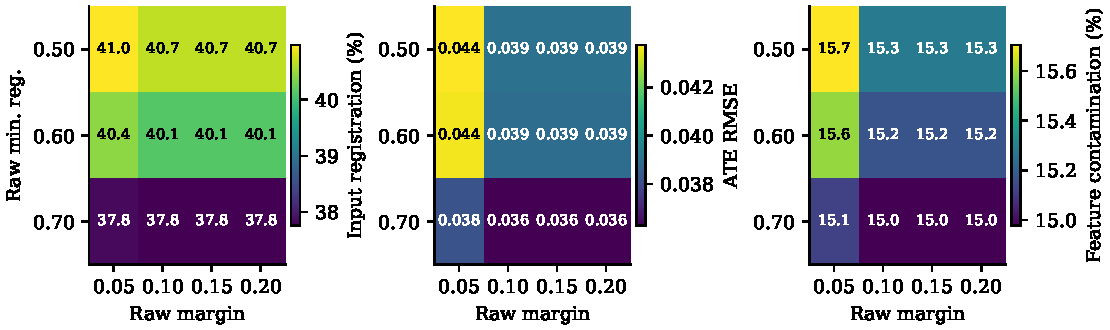
\includegraphics[width=\linewidth]{figures/aqua_paper_tables/fig_r099_sensitivity.pdf}
\caption{Sensitivity of the R099 raw-fallback selector over neighboring raw-registration thresholds and margins. The pose-evaluation success stays fixed at 90.28\% across all twelve settings; the figure shows the remaining registration, ATE, and contamination variation.}
\label{fig:aqua_r099_sensitivity}
\end{figure}
